\chapter{Methodology}
\index{Methodology@\emph{Methodology}}%
\label{chap:methodology}

\section{Overview}\label{sec:method overview}

To examine the effects of cooperativity conscious schedulers we needed to have 
a method for comparing several scheduler implementations without needing to 
modify the underlying implementation of processes, channels, or application
source code. It would be also beneficial if our solution were able to visualize
these differences similar to Haskell's ThreadScope \cite{jones2009parallel}.

Our solution, $ErLam$, is a compiler for an experimental version of Lambda 
Calculus with Swap Channels and a runtime system which allows for swappable 
scheduler mechanisms and an optional logging system which can be fed into a 
custom report generator.
We break up our solution description into three parts; 
Section~\ref{sec:erlam}
will duscuss our language syntax and semantics. It will also demonstrate our
Runtime Scheduler API by breaking down the CML Interactivity scheduler. 
Section~\ref{sec:simulation and visualization} 
will go more into depth about
our testing environment which involves our logging system, the report generator,
and the set of example applications we used to represent different cooperativity
levels. 
Finally, Section~\ref{sec:cooperativity mechanics} will go over our
example schedulers we wrote which demonstrate cooperative-conscious behavior. 
These will be the schedulers we provide our results against.

\section{ErLam}\label{sec:erlam}

The ErLam toolkit is itself broken down into three parts, the language and its
semantics, the Runtime System, and the Scheduler API. We will first lay out the
language and it's basic semantics, as the finer-details are reliant on the exact
selected scheduling solution as well as the chosen swap-channel implementation.
We will then examine the possible channel implementations and how they effect
the given semantics. Finally we will discuss the Scheduler API using an example
scheduler implementation.

\subsection{The ErLam Language}\label{sec:the erlam language}

The ErLam Language is based on Lambda Calculus, with first-class single 
variable functions, but deviates somewhat in that it provides other first-class 
entities. It deviates from Church representation to provide Integers, this is
purely for ease of use. It also provides a symmetric synchronous Channel type 
for interprocess communication. As a note, this language can also be classified 
as a Simply-Typed Lambda Calculus.

ErLam also makes a number of ease-of-use decisions like providing a default 
branch operator and has some useful syntactic sugar such as SML style $let$ 
expressions and multi-variable function definitions. There is also a set of
built in functions for numeric operations, type checking, and standard 
functional behaviors (\eg~combinators, \etc) which are ignored in this 
document.

\begin{figure} %% THE ERLAM LANGUAGE BNF WITHOUT SYNTAX SUGAR %%
\centering
{\footnotesize
    %%
%% ErLam BNF Style Grammar.
%%
\begin{BVerbatim}[commandchars=\\\{\}]
<Expression> ::= <Variable> 
              |  <Integer>
              |  `\textbf{newchan}'
              |  `\textbf{(}' <Expression> `\textbf{)}'
              |  <Expression> <Expression>
              |  `\textbf{if}' <Expression> <Expression> <Expression>
              |  `\textbf{swap}' <Channel> <Expression>
              |  `\textbf{spawn}' <Expression>
              |  `\textbf{fun}' <Variable> `\textbf{.}' <Expression>
\end{BVerbatim}

}
\caption{The ErLam language grammar, without syntax sugar or types.}
\label{fig:grammer}
\end{figure}

Figure~\ref{fig:grammer} expresses ErLam in its simplified BN-Form. The 
semantics for the language is fairly straight forward, but it's operational 
semantics are layed out in appendix~\ref{app:semantics}. All expressions reduce
to one of the terminal types: Integer, Channel, or Function. To spawn for 
instance, if any terminal is passed other than a function, it returns a $0$
(\eg~false). When the function is passed, it is applied with $nil$ to 
initialize the internal expression. 

ErLam extends this grammar only a little to add SML style $let$ expressions and
multiple variable functions which are curried from left to right (see 
figure~\ref{fig:sugar-transform} for syntactic transformation). We will be using
this syntactic sugar throughout this document to make our source easier to 
review.

\begin{figure}
    \centering
    \[
        \textbf{let}\: x\: =\: e_1\: \textbf{in}\: e_2
        \Rightarrow
        ((\textbf{fun}\: x.e_2)\; e_1)
    \]
    \[
        \textbf{fun}\: \textit{x,y,z} . \textit{e}
        \Rightarrow
        \textbf{fun}\: \textit{x} . (\textbf{fun}\: \textit{y} . (\textbf{fun}\: \textit{z} . \textit{e} ))
    \]
    \caption{Syntactic sugar parse transformations.}
    \label{fig:sugar-transform}
\end{figure}

Also, note the possible steps $\textbf{swap}$ can take: either returning the 
null set or another expression and a set of functions. In the former's case, 
the channel has blocked and the only course of action is to get another 
expression to work on from the scheduler. In the later's case, we have an
expression to work on, but we also may have unblocked other processes in the
process so we need to reschedule them. 

Note however, that return set may be null and the expression returned may be
another attempt at swapping (\ie~$e = (\textbf{swap}\:c\:v)$). This would let 
the scheduler choose whether to retry immediately or reschedule it for a later
time and work on something in the mean time.

\subsection{Channel Implementations}\label{sec:channel implementations}

ErLam provides a selection of channel implementations so as to allow for 
interchangable comparisons to be made with synchronization methods and the 
schedulers themselves. ErLam comes with two channel implementations the 
{\sl Blocking} Swap, and the {\sl Absorbing} Swap. 
We will now look at an example application and it's execution
using both methods for comparison.

\begin{wrapfigure}{r}{0.5\textwidth}
    \centering
\begin{BVerbatim}[commandchars=\\\{\}]
\textbf{let} c = \textbf{newchan in}
\textbf{let} f = (\textbf{fun} _.(\textbf{swap} c \textit{42})) \textbf{in}
\textbf{let} _ = (\textbf{spawn} f) \textbf{in}
\textbf{in} (\textbf{swap} c \textit{0})
\end{BVerbatim}
    \caption{A simple ErLam application which swaps on a channel before returning.}
    \label{fig:swap-example}
\end{wrapfigure}

Figure~\ref{fig:swap-example} gives an example ErLam application. It first 
creates a new channel for processes to communicate on. It then creates a 
null-function to spawn, who's sole purpose is to swap on the channel the number
$42$ and then die. Finally, it swaps on the channel the number $0$ and returns
the result of the whole evaluation, which in this case will be the value passed
from the other end of the swap, $42$. 

As ErLam is innately concurrent, we do not know which process will ask to swap
first. It may even be possible that $0$ asks to swap several times before $42$
even tries. In fact, the {\sl Blocking} channel allows multiple swap attempts,
We can see an illustration of this in figure~\ref{fig:blockchan-example}; note
the illustration makes no mention of the scheduler or it's functionality. It may
be the case that the two processes are on different processing units and are in
different process queues. Or it may be the case that they both exist in the
same queue and upon a block, the scheduler chooses the next one, which will 
immediately unblock the channel.

\begin{figure}
    \makebox[\textwidth][c]{
\subfigure[t][Process Blocking Swap]{
    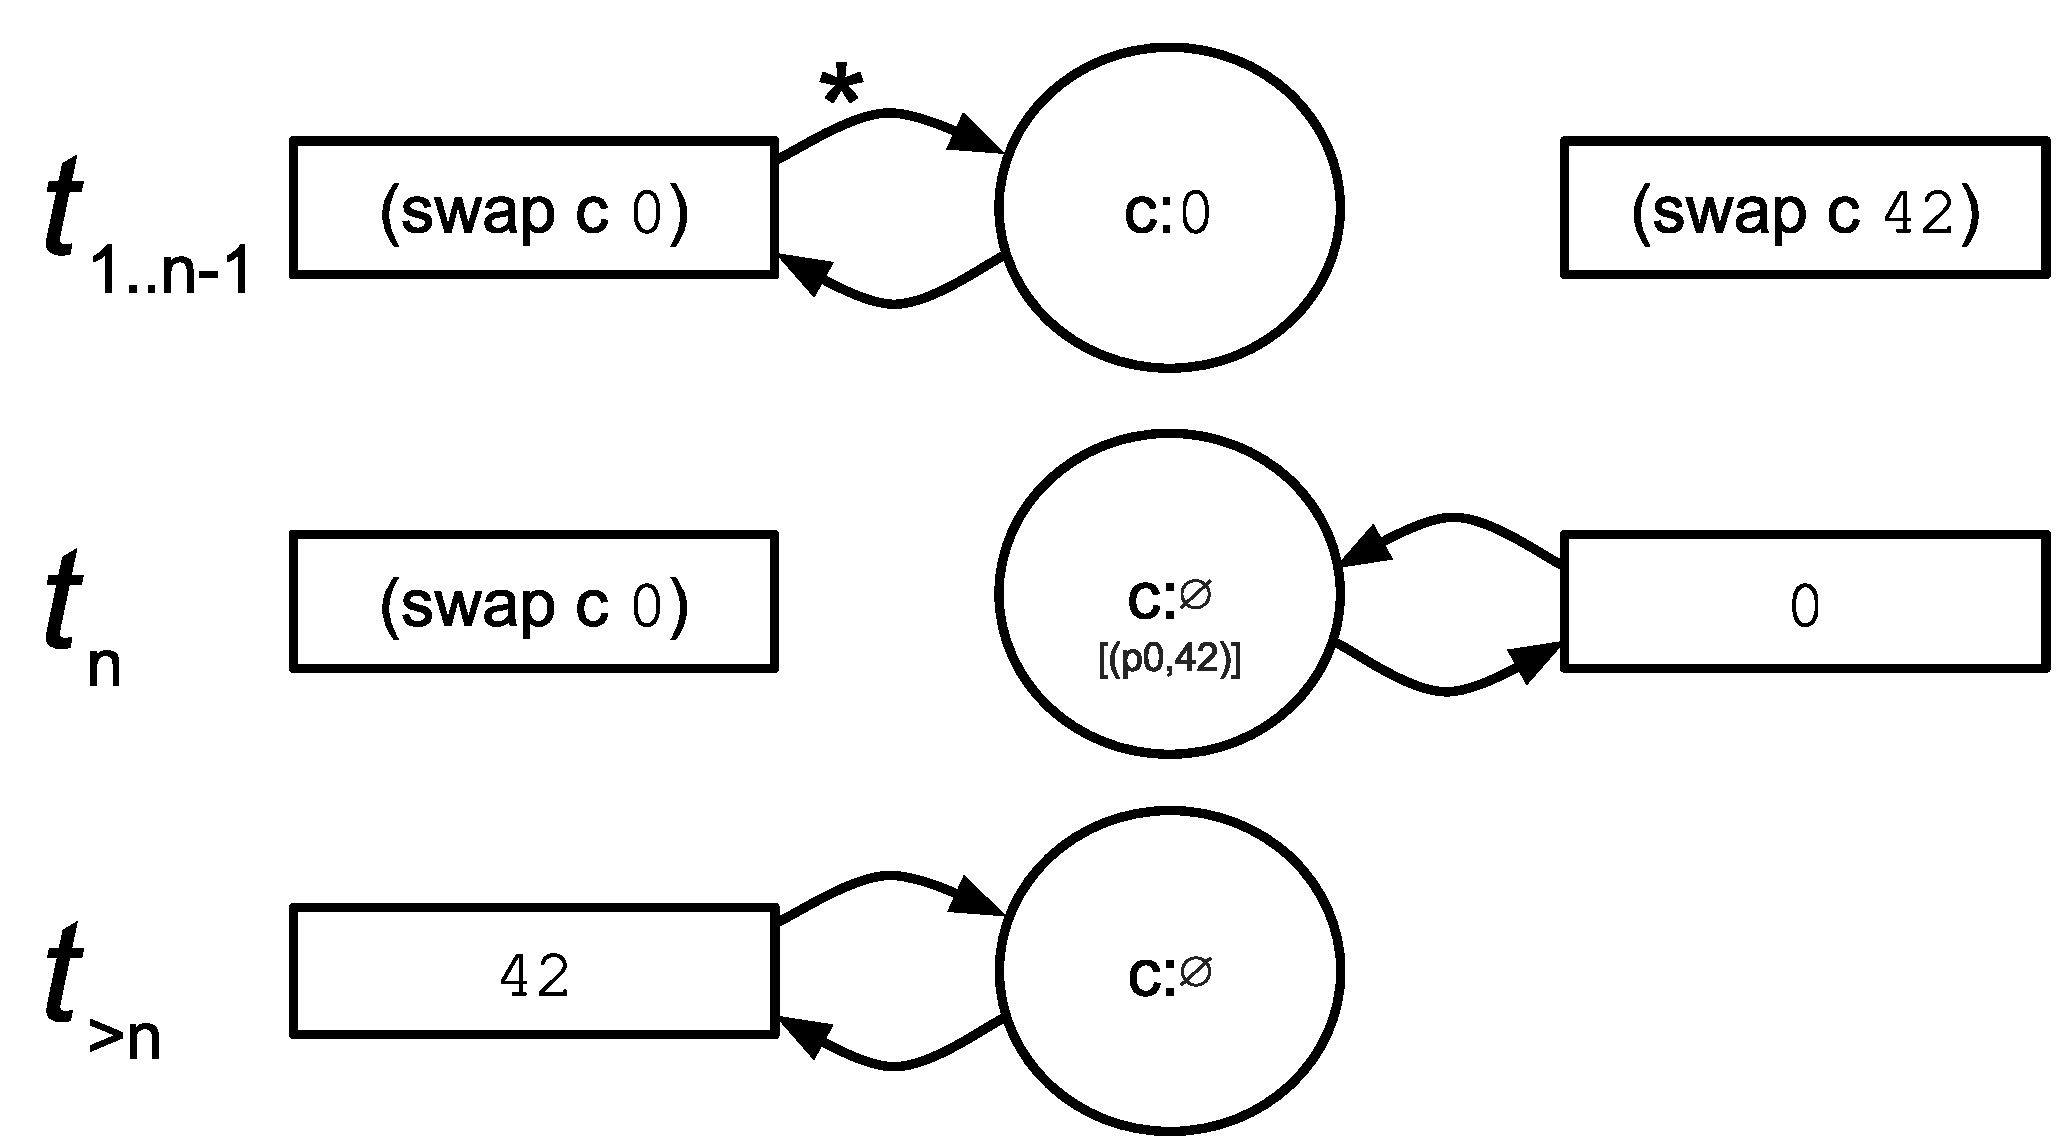
\includegraphics[scale=0.25]{BlockingSwap.pdf}
    \label{fig:blockchan-example}
}  \subfigure[t][Process Absorption Swap]{
    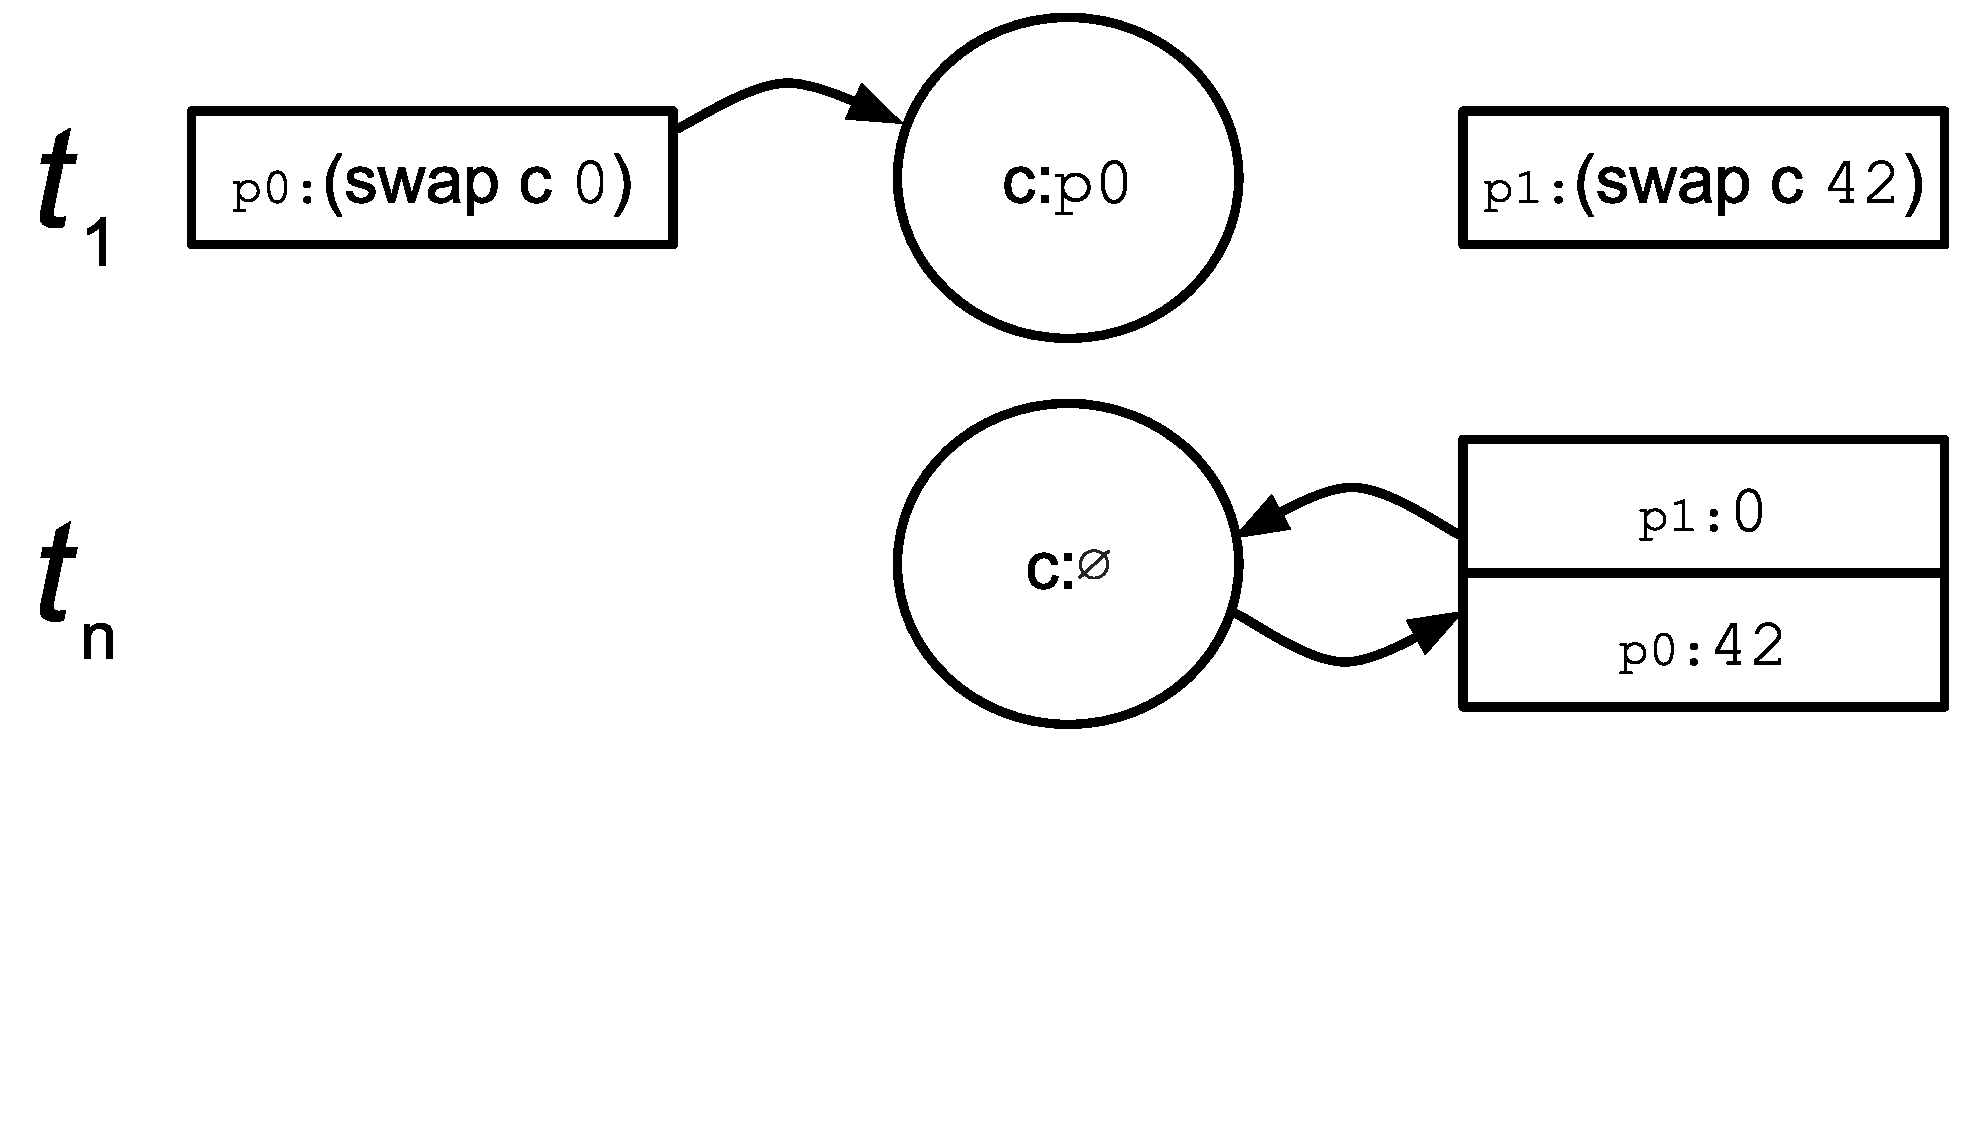
\includegraphics[scale=0.25]{AbsorbSwap2.pdf}
    \label{fig:absorbchan-example}
}}
\caption{Channel operation over time. Note abitrary time-slice $t_1$ is when the 
first swap operation is evaluated.}
\end{figure}

The {\sl Blocking} channel effectively simulates a common spin-lock over a shared 
piece of memory. These channels represent a worst-case, albeit common, application 
implemenatation for concurrent software. Even so, they do allow for some hints
to the scheduler, which can be taken advantage of. Alternatives on the spin-lock 
could be added to the ErLam toolkit though, such as a push-notifying semaphore, 
however we provide a simpler and functionally more common alternative: the process 
absorption channel.

In the {\sl Absorption} channel (figure~\ref{fig:absorbchan-example}), the first 
process to get to the channel will get absorbed by it. The scheduler in 
question will be out a process, and but the scheduler which unblocks the channel 
by arriving second will get back two processes (the one performing the swap, 
and the absorbed one). In terms of scheduling efficiency this type of message
passing channel has provideded enormous improvements for runtimes which do not
wish to introduce channel inspection into their scheduler.

%This channel implementation gets closer to taking advantage of
%cooperativity as it will relocate communicating processes to the scheduler 
%which has another process to unblock it. But with this comes the added overhead 
%of relocating processes and if the scheduler uses a single queue there is no
%added benefit (at least with $swap$ channels). 

\subsection{The Scheduler API}\label{sec:the scheduler api}

ErLam was written in Erlang, and as such, it takes advantage of Erlang's 
callback behaviour specifications. An \emph{erlam\_scheduler} behaviour has been 
defined which requires a minimalistic $5$ callback functions 
(figure~\ref{fig:scheduler-api}).

\begin{figure}
    \begin{minted}[frame=lines,fontsize=\footnotesize]{erlang}
-callback layout( erlang:cpu_topology(), scheduler_opts() ) -> 
                scheduler_layout().

-callback init( scheduler_opts() ) -> 
                {ok, scheduler_state()} |
                {error, log_msg()}      |
                {warn, log_msg(), scheduler_state()}.

-callback cleanup( scheduler_state() ) -> 
                ok | {error, log_msg()} | {warn, log_msg()}.

-callback tick( scheduler_status(), scheduler_state() ) -> 
                {ok, scheduler_status(), scheduler_state()} |
                {return, term()} | {stop, scheduler_state()}. 

-callback spawn_process( erlam_process(), scheduler_state() ) -> 
                {ok, scheduler_state()} | {error, log_msg()}.
\end{minted}
\caption{The ErLam Scheduler API}
\label{fig:scheduler-api}
\end{figure}

Upon instantiation of the runtime the runtime system will call the 
\emph{layout/2} function with the NUMA layout of the system the application is
running on, along with any parameters the user specified at runtime. The 
result of this function is to be the scheduler layout. 

For example, let's assume we are running our application on a Intel Core i7 
which has 4 logical cores which support hyperthreading. The \emph{layout/2}
function will be given the following structure: 

{\footnotesize 
\begin{verbatim}
   [{processor,[{core,[{thread,{logical,0}},{thread,{logical,1}}]},
                {core,[{thread,{logical,2}},{thread,{logical,3}}]},
                {core,[{thread,{logical,4}},{thread,{logical,5}}]},
                {core,[{thread,{logical,6}},{thread,{logical,7}}]}]}].
\end{verbatim}
} 

\noindent
This indicates to the scheduler implementation that it at max, can spawn $8$
instances of itself which would be bound to each logical processing unit (LPU).
We could of course have a scheduler which acts differently based on how the
architecture. However, the schedulers we have limited ourselves to are either
single or fully multi-core (\ie~uses all available LPUs).

To spin up an instance of the scheduler on the particular core, the 
\emph{init/1} function is called which should return the scheduler's state. 
As Erlang is a functional language, we use this state object as a means to
maintain some global state for each scheduler process by threading it through
all subsequent callback calls. Upon shutdown, the oposite function 
\emph{cleanup/1} is called.

The last two functions are the most interesting as they pertain to the core of
what each new scheduler provides, namely how to evaluate the world in a given
timeslice (\emph{tick/2}) and how a new process should be handled 
(\emph{spawn\_process/2}); but an explaination of these callbacks is best done 
through example.

\subsection{Example: The CML Scheduler}\label{sec:example the cml scheduler}

Concurrent ML is an extention to SML which adds the \emph{spawn} function, and 
channel operations. CML's scheduler utilizes a dual-queue structure rather than
a simple unary-process-queue. The scheduler attempts to differentiate between
{\em communication} and {\em computation}-bound processes so as to reduce the
effects of highly computationally intensive processes from choking the system.
The scheduling system thus improves on application interactivity by demoting 
{\em computation}-bound processes to the secondary queue (which isn't accessed
until another process is demoted).

Spawning a process in the CML scheduler (figure~\ref{fig:cml-spawn-process}) 
does not go onto the primary queue, instead we enqueue the current process and 
start evaluating the new process. This is a fairly simplistic example, but it 
shows how one would go about updating the state between ticks.

\begin{figure}
\begin{minted}[frame=lines,fontsize=\footnotesize]{erlang}
spawn_process( Process, State ) -> 
    enqueueAndSwitchCurThread( Process, State ).

enqueueAndSwitchCurThread( Process, #state{curThread=T}=State ) ->
    case T of
        nil ->
            setCurThread( Process, State );
        _   ->
            % New process takes over
            {ok, NewState} = enqueue1( T, State ), 
            setCurThread( Process, NewState )
    end.
\end{minted}
\caption{CML Process Spawning.}
\label{fig:cml-spawn-process}
\end{figure}

In the original CML scheduler, it defined a quantum which it would let the 
current process run for, and then it would preempt it if it attempted to run 
for longer. The ErLam runtime avoids the use of time based quantum as logging 
and other factors directly effect the usefulness of this. Instead it uses a 
'tick', which is suppose to emulate one
step forward in the execution of the application. Thus to simulate a quantum we
instead keep track of the number of reductions performed on the current process
and decrement the counter until we reach 0.

\begin{figure}
\begin{minted}[frame=lines,fontsize=\footnotesize]{erlang}
tick( _Status, #state{ curReduct=0 }=State ) ->
    {ok, NState} =  pick_next( State ),
    reduce( NState );
tick( _Status, State ) -> reduce( State ).

pick_next( State ) ->
    {ok, NewState} = preempt( State ),      % Place cur thread onto queue
    {ok, Top, Next} = dequeue1( NewState ), % Pop next off
    setCurThread( Top, Next ).              % Set as cur and return state
\end{minted}
\caption{CML Process evaluation.}
\label{fig:cml-tick}
\end{figure}

The \emph{tick/2} function (figure~\ref{fig:cml-tick}) performs one of two 
things based on what the state of the system is. If the current reduction count 
is $0$, then we can pick a new process from the queue, otherwise we can perform
a reduction. 

Note for our scheduler simulation we ignore the first parameter to the 
\emph{tick/2} function for either case. The first parameter was the status of 
the scheduler returned from the previous tick (\eg~running, waiting, \etc). This 
would be useful if the CML scheduler utilized work-stealing to get work to do
from other LPUs when in \emph{waiting} mode.

\subsection{Provided Schedulers}

Along with the Single-Threaded Dual Queue CML scheduler {\sl (STDQ)}, ErLam 
comes with several basic scheduling mechanics. We utilize these as bases cases 
on which to compare the behaviour of all subsequent feedback-enabled schedulers.

\begin{itemize}
    \item {\bf The Single-Threaded Round-Robin Scheduler {\sl (STRR)}} \\
        This scheduler uses a single FIFO queue which all processes are spawned 
        to. There is no rearrangement of order, and the single-thread scheduler 
        will just round-robin the queue performing a set number of reductions
        per process before enqueuing and poping the next one.

    \item {\bf The Multi-Threaded Round-Robin Global-Queue Scheduler {\sl (MTRRGQ)}} \\
        A multi-core version of the previous scheduler. This uses a single global
        process queue which all schedulers share and attempt to work from.

    \item {\bf The Multi-Threaded Round-Robin Work-Stealing Scheduler {\sl (MTRRWS)}} \\
        An improvement on the previous scheduler. Instead of a global process 
        queue, each scheduler maintains their own. A waiting scheduler will randomly 
        sleep-and-steal until it finds a process to work on from another scheduler. 
        The provided implementation gives two example stealing mechanisms:
        \begin{itemize}
            \item {\bf Shared-Queue {\sl (MTRRWS-SQ)}} \\
                Stealing a process involved performing an atomic dequeue from 
                the bottom (rather than the top) of another scheduler's process 
                queue. This will only block the other scheduler from performing
                a dequeue for a very short window of time, but involves 
                accessing "remote" memory.
            \item {\bf Interrupting-Steal {\sl (MTRRWS-IS)}} \\
                Simulates sending an evil theif-process over to another scheduler.
                When the victim scheduler preempts or yields their current process
                and selects the next one from the queue, they will instead get a
                theif process which will syphon a process away to the theif's home
                scheduler.
        \end{itemize}
\end{itemize}

ErLam also comes with three cooperativity-conscious schedulers: the 
Longevity-Based Batching Scheduler (section~\ref{sec:longevity based batching}),
the Channel Pinning Scheduler (section~\ref{sec:channel pinning}), and the
Bipartite Graph Aided Shuffling Scheduler (section~\ref{sec:bipartite graph aided shuffling}).
The first two build on the same shared queue module as provided by $MTRRWS^{\*}$, 
while the third utilizes it's own implementation.

\section{Simulation \& Visualization}\label{sec:simulation and visualization}

The second primary goal of the ErLam toolkit was the ability to visualize 
how the scheduler proceeded to evaluate a simulated application. Thus we needed
a way to log all events over time, including unique per-scheduler events, such 
as the size of both the primary and secondary queues in the CML scheduler.

As a secondary goal, we need a sample set of application simulations to run 
against our set of schedulers. These simmulations would need to be concise and
demonstrate various levels of cooperativity and phase changes. We would like
to also have the ability to mix and match test cases together to better create
realistic work-sets for the schedulers to react to.

\subsection{Runtime Log Reports}\label{sec:runtime log reports}

Logging in Erlang is a fairly simple matter. We utilize a simplistic data 
logging module based on syslog. The output of running an application 
could look like this:
{\footnotesize
\begin{verbatim}
                    timestamp,lpu,event,value
                    ...
                    983847.935268,3,sched_state,running
                    983847.935333,0,queue_length,59
                    983847.935677,24,channel_blocked,6102
                    983847.935683,6,yield,""
                    983847.936003,0,queue_length,59
                    983847.936430,3,tick,""
                    983847.936439,3,reduction,""
                    ...
\end{verbatim}
}
\noindent
The timestamp given is a concatenation of the second and microsecond that the
event happened in. The lpu is the scheduler which caused the event, unless it's
a channel based event, such as a \emph{channel\_blocked} event, in which case it's
the channel ID. 

Our logging API is fairly simplistic as we only need to capture two types of metrics
from our events: quantity and frequency. With frequency, we want to know the
amount of events which happened in a time range, but with quantity we would like 
things like length of the scheduler's process queue over time or the amount of
time spent in the running or waiting state.

Note time is not consistent per LPU, it may be the case that another OS 
application is getting time instead of one of the ErLam schedulers. This could
result in one or more of the LPUs getting far less \emph{``tick''} events. Worse
yet, there may be a large gap of time missing from one scheduler to the next.
For our purposes though we would like to compare the state of the scheduler
while it is executing and would be fine with averaging over the largest gap. These
from experimentation have not been found to be very frequent or large on an
otherwise unoccupied processor.\todo{Anecdotal! I need to prove this}

To explain this averaging technique we'll now discuss the report generation 
method. The ErLam toolkit comes with a secondary R script which can be given a 
generated log file for processing. This script dynamically loads chart 
creation scripts based on the types of events it sees in the log file. The
toolkit comes with five charting scripts which should work for all schedulers: 
Channel Usage (Communication Density) over time,
Channel State (blocked vs. unblocked) over time,
Process Queue Length per LPU over time,
Reductions (Computation Density) over time, and
Scheduler State (running vs waiting) over time.

\begin{wrapfigure}{r}{0.5\textwidth}
\centering
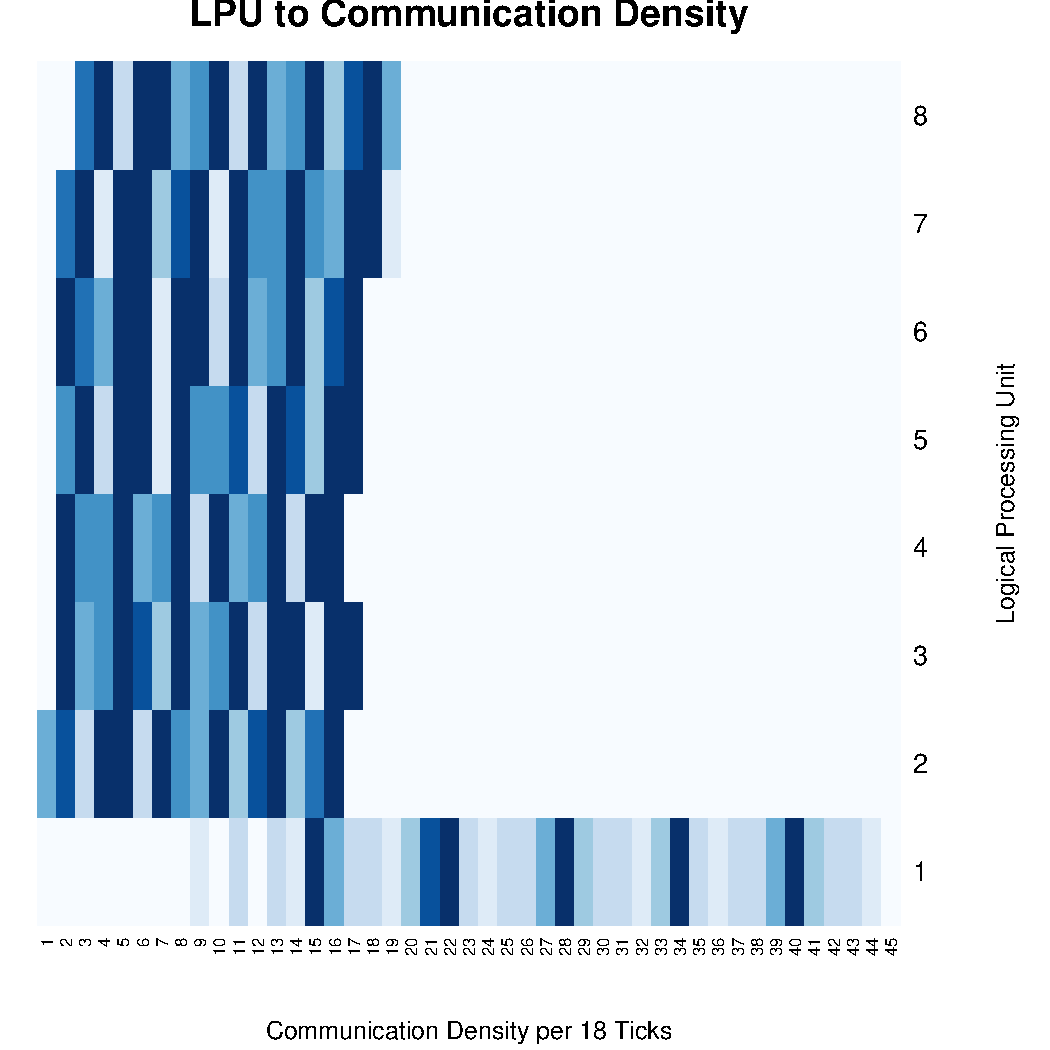
\includegraphics[scale=0.35]{pring-erlam_sched_multi_ws-commdense.pdf}
\caption{\footnotesize Example of Communication Density graph for the Work-Stealing scheduler 
on a Core i7 running the $PRing$ application.}
\label{fig:commdense-example}
\end{wrapfigure}

Communication Density for example (see figure~\ref{fig:commdense-example}, 
creates a heatmap based on the frequency of
\emph{yield} events which occur whenever a process attempts a $swap$. Each cell
of the heatmap is a color intensity based on the number of \emph{yield} events 
seen in a given timeslice for a given LPU. This timeslice is where the averages
come into play. R heatmaps have a max number of colors of $9$, so any range we 
select must be modulo $9$. However, the constant multiplicand is based on the
mean amount of time $N$ ticks take place accross each LPU.
We can obviously tune the accuracy of these averages on a per-LPU basis by
modifying $N$. Anecdotally, this turned out to be adventagous on several 
occasions when debugging scheduler implementations. As decreasing the number of
ticks to average for, pushed the number of samples (and thus accuracy) higher.

\subsection{Cooperativity Testing}\label{sec:cooperativity testing}

As part of the thought experiment, we needed to implement a decent set of test 
cases which would give us a good coverage of the range of cooperative behaviour
in our applications. 

On one hand we have an axis depicting the amount of parallelism possible in our 
application. A system which is completely parallel, would be one where all 
processes spawned have no dependence on any of the others. For our toolkit, we 
called this behaviour $ChugMachine_N$ (figure~\ref{fig:ChugMachine}) ; where $N$ depicts the number of parallel 
processes. On the other side of the axis, we would have a system which had 
absolutely no parallelism possible. We called this behaviour $PRing_N$ (figure~\ref{fig:PRing}), as it
would spawn $N$ processes in a ring formation and pass a token in one direction.
Each process has a channel to its left and right and would synchronize to the 
right until it recieves a token to continue. 

$PRing_N$ also gives an example of full-system cooperation, except we would 
instead like some degree of parallelism possible. To expirement with that, we 
would have to throttle the degree of cooperativity. This behaviour is called
$ClusterComm_{(N,M)}$ (figure~\ref{fig:ClusterComm}) as it spawns $N$ processes and $M$ channels which can be
synchronized with by any process. Note for this system to work with swap 
channels we limit $M$ to be at most $\lfloor N/2 \rfloor$ for all tests. 

$ClusterComm_{(N,M)}$ is also an example of full-system cooperation, we also
want to have a possible case for partial-system cooperation. We begin this range
of experiments with a behaviour which acts like a bunch of $ClusterComm_{(N,1)}$
running in parallel. We call this special case behaviour $PTree_W$ (figure~\ref{fig:PTree}); where $W$ is 
the number of work groups to run in parallel. This is the cleanest case of 
partial-system cooperation. We would expect to see obvious clustering of 
processes by work-group affiliation if the scheduler was 
cooperativity-conscious.

However, to expand on the concept of partial-system cooperativity, we would 
also like to experiment with lop-sided behaviours where a work-group exists 
along with other processes which may not be affiliated with one another. An 
application like this would be the combination of $ClusterComm_{(N,M)}$, 
$ChugMachine_N$, and $PRing_N$ running in parallel.

We are missing two important behaviour simulations: application phase changes,
and hanging processes (typical of I/O bound processes). In the case of the 
latter, a simple built-in command $hang$ was provided which would simulate 
hanging for a random amount of time before allowing the process to proceed with
evaluation. If a scheduler attempted to reduce the process before the $hang$ 
time was completed, it would be immediately preempted. The behaviour 
implemented we call $UserInput_{(T,C)}$ (figure~\ref{fig:UserInput}); where $T$ is the max time in seconds
the process would hang before continuing, and $C$ is the number of times it 
would simulate ``waiting for user input''.

For the former missing behaviour, phase changes, we decided to make a variation
of $PTree_W$ called $JumpShip_{(W,P)}$ (figure~\ref{fig:JumpShip}) which would act like $PTree_W$ but would
``change phase'' $P$ times before completion. The act of ``changing phase'' would 
be the successive relocation of all the processes from one work-group to 
another, effectively having all processes from work-group $X$ ``jump-ship'' to
$X+1$ \textbf{mod} $N$.

We would have liked to possibly experiment with variations on the ``jump-ship''
behaviour so as to inject phase changes into $PRing_N$ (by perhaps reversing
direction) or $ClusterComm_{(N,M)}$ (by switching to $ChugMachine_N$ for a 
brief period before returning to $ClusterComm_{(N,M)}$).

\begin{figure}
\subfigure[t][Graphical representation of $PTree$, $N$ Parallel work groups.]{
    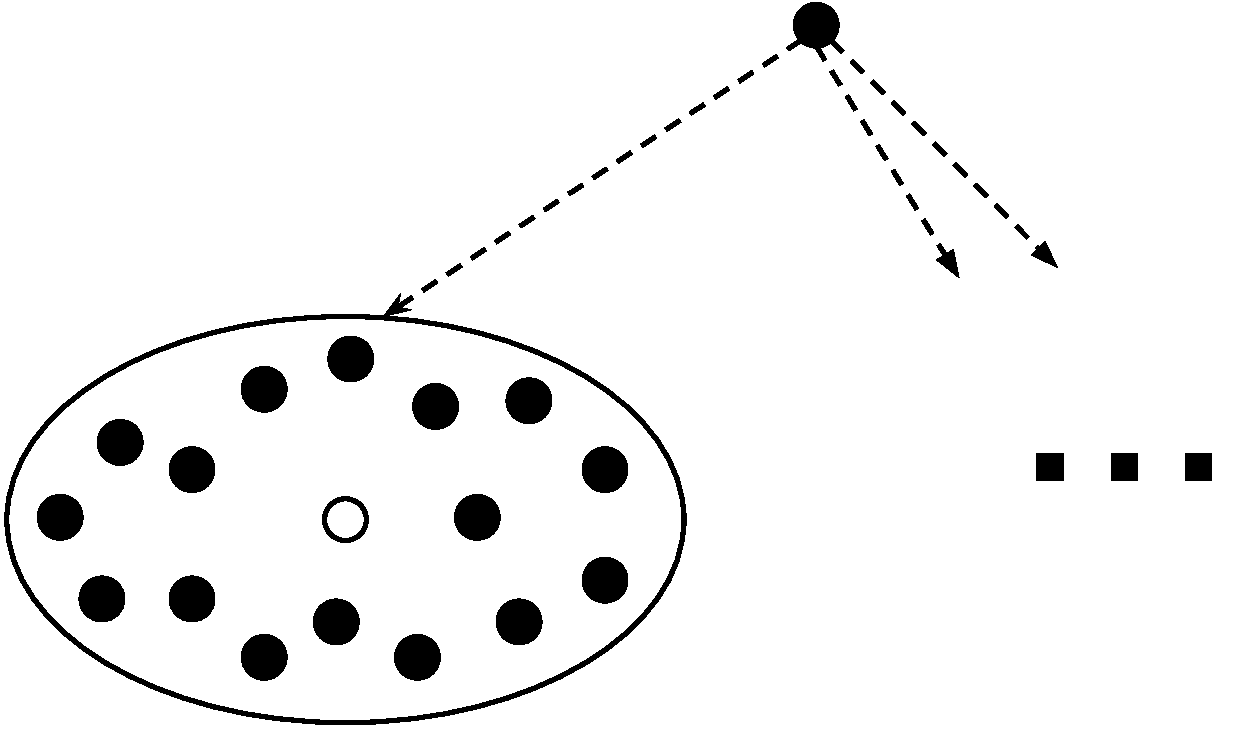
\includegraphics[scale=0.35]{PTree.pdf}
    \label{fig:PTree}
} 
\hfill
\subfigure[t][Graphical representation of $PRing$, full system predictable cooperation.]{
    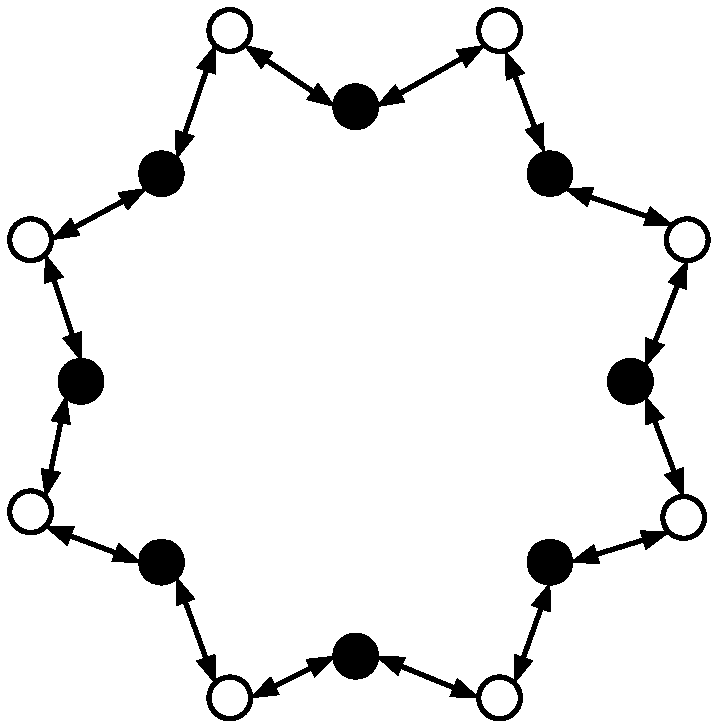
\includegraphics[scale=0.35]{PRing.pdf}
    \label{fig:PRing}
}

\subfigure[t][Graphical representation of $ClusterComm$, $N$ processes to $M$ channels for unpredictable full system cooperation.]{
    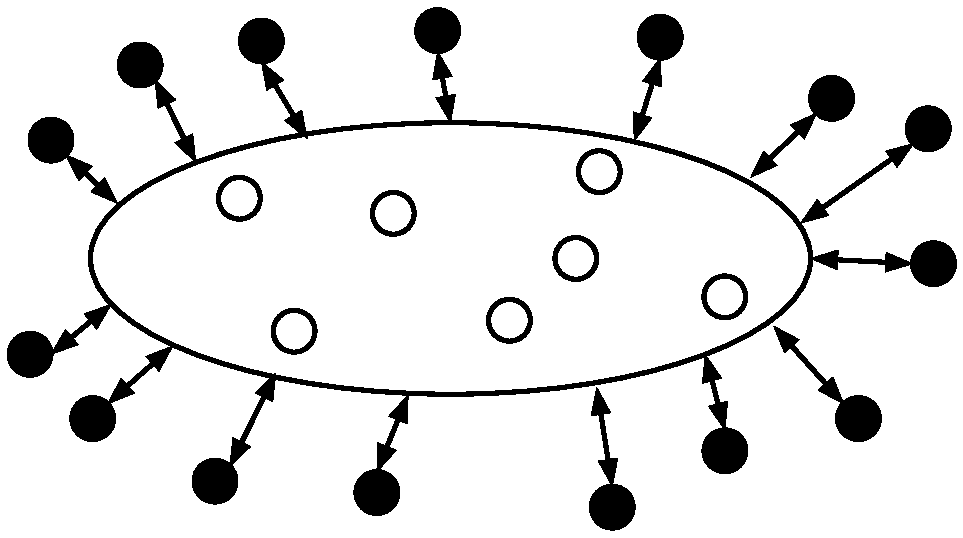
\includegraphics[scale=0.35]{ClusterComm.pdf}
    \label{fig:ClusterComm}
}
\hfill
\subfigure[t][Graphical representation of $ChugMachine$, $N$ worker processes without cooperation.]{
    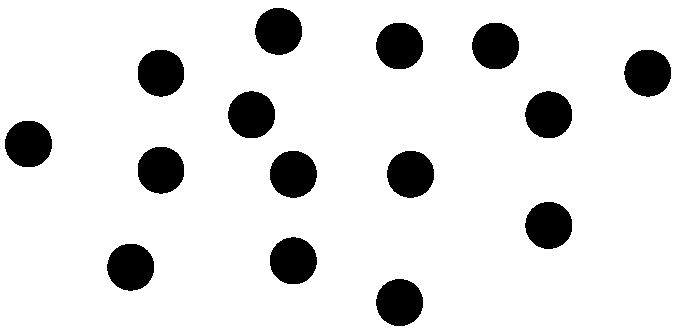
\includegraphics[scale=0.45]{ChugMachine.pdf}
    \label{fig:ChugMachine}
}

\subfigure[t][Graphical representation of $UserInput$, single randomly hanging process.]{
    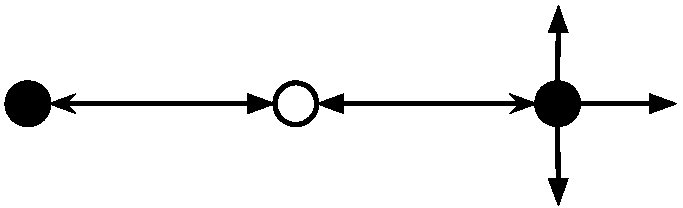
\includegraphics[scale=0.55]{UserInput.pdf}
    \label{fig:UserInput}
}
\hfill
\subfigure[t][Graphical representation of $JumpShip$, $N$ Parallel phase shifting work groups.]{
    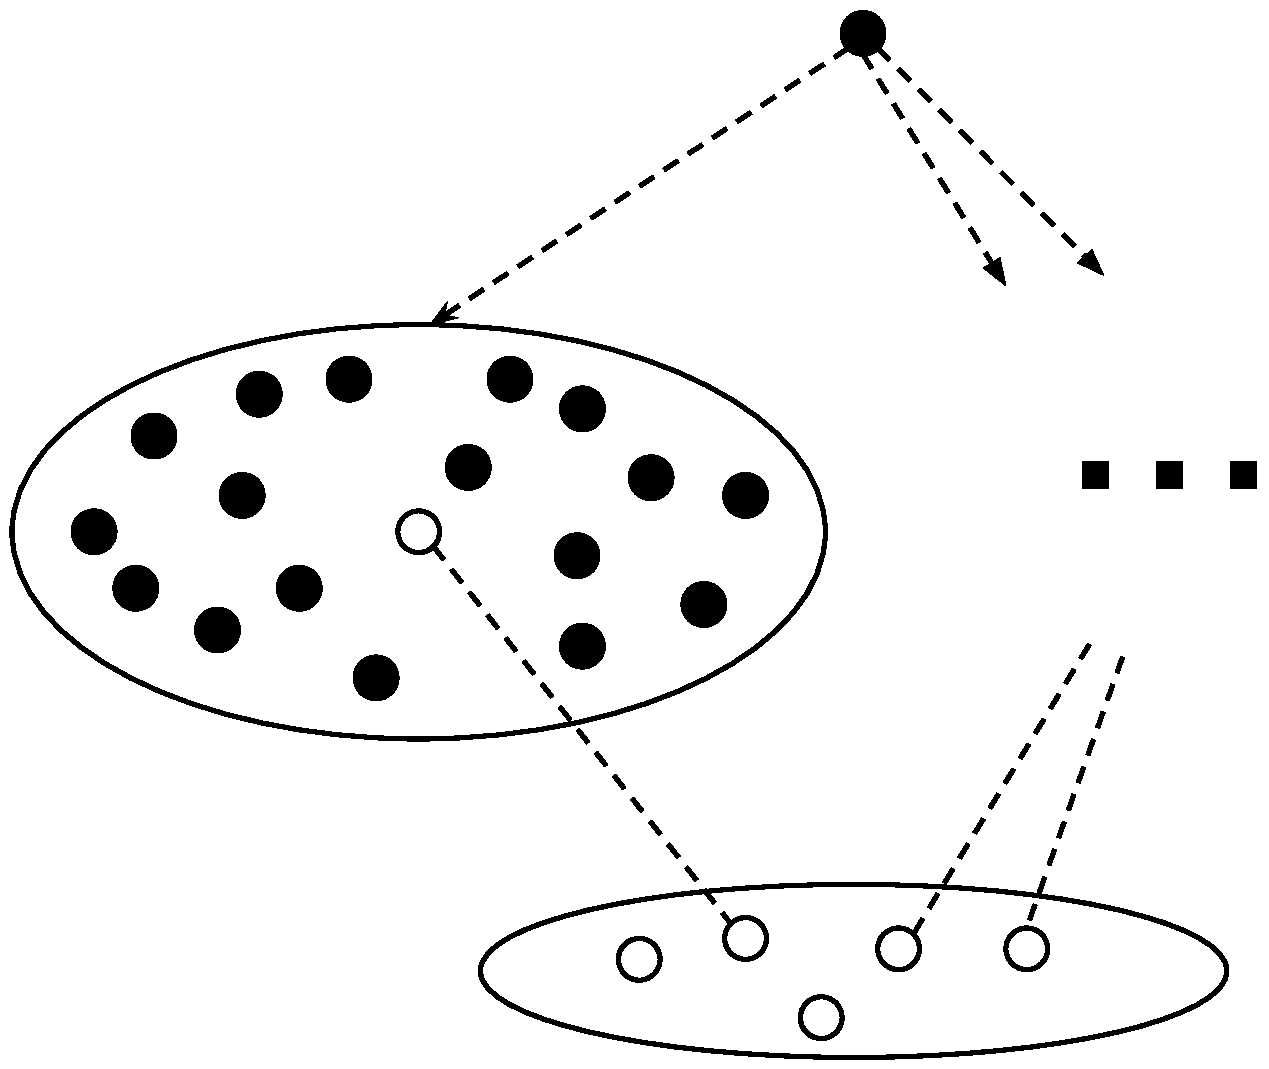
\includegraphics[scale=0.35]{JumpShip.pdf}
    \label{fig:JumpShip}
}
\caption{Simulated behaviour examples.}
\end{figure}


\section{Cooperativity Mechanics}\label{sec:cooperativity mechanics}

As mentioned previously, ErLam provides a number of feedback-enabled 
cooperativity-conscious schedulers for comparison purposes. However, before a
detailed description of their function, we will discuss an overview of practical
cooperativity recognition as well as our approach to designing mechanisms to
take advantage of it.

\subsection{Overview \& Approach}\label{sec:cooperativity mechanics overview}


Approach: 


\subsection{Longevity-Based Batching}\label{sec:longevity based batching}



\subsection{Channel Pinning}\label{sec:channel pinning}




\subsection{Bipartite Graph Aided Shuffling}
    \label{sec:bipartite graph aided shuffling}


